\documentclass[9pt,twocolumn,twoside,lineno]{pnas-new}

% Use the lineno option to display guide line numbers if required.
% Note that the use of elements such as single-column equations
% may affect the guide line number alignment.


\usepackage[T1]{fontenc}
\usepackage[utf8]{inputenc}

% tightlist command for lists without linebreak
\providecommand{\tightlist}{%
  \setlength{\itemsep}{0pt}\setlength{\parskip}{0pt}}


% Pandoc citation processing
\newlength{\cslhangindent}
\setlength{\cslhangindent}{1.5em}
\newlength{\csllabelwidth}
\setlength{\csllabelwidth}{3em}
\newlength{\cslentryspacingunit} % times entry-spacing
\setlength{\cslentryspacingunit}{\parskip}
% for Pandoc 2.8 to 2.10.1
\newenvironment{cslreferences}%
  {}%
  {\par}
% For Pandoc 2.11+
\newenvironment{CSLReferences}[2] % #1 hanging-ident, #2 entry spacing
 {% don't indent paragraphs
  \setlength{\parindent}{0pt}
  % turn on hanging indent if param 1 is 1
  \ifodd #1
  \let\oldpar\par
  \def\par{\hangindent=\cslhangindent\oldpar}
  \fi
  % set entry spacing
  \setlength{\parskip}{#2\cslentryspacingunit}
 }%
 {}
\usepackage{calc}
\newcommand{\CSLBlock}[1]{#1\hfill\break}
\newcommand{\CSLLeftMargin}[1]{\parbox[t]{\csllabelwidth}{#1}}
\newcommand{\CSLRightInline}[1]{\parbox[t]{\linewidth - \csllabelwidth}{#1}\break}
\newcommand{\CSLIndent}[1]{\hspace{\cslhangindent}#1}


\templatetype{pnasresearcharticle}  % Choose template

\title{Environmentally robust \emph{cis}-regulatory changes underlie
rapid climatic adaptation}

\author[a,b,1,2]{Mallory A. Ballinger}
\author[c,1]{Katya L. Mack}
\author[a,b]{Sylvia M. Durkin}
\author[a,d]{Eric A. Riddell}
\author[a,b,2]{Michael W. Nachman}

  \affil[a]{Museum of Vertebrate Zoology, University of California,
Berkeley, Berkeley, CA, 94720}
  \affil[b]{Department of Integrative Biology, University of California,
Berkeley, Berkeley, CA, 94720}
  \affil[c]{Department of Biology, Stanford University, Stanford, CA,
94305}
  \affil[d]{Department of Ecology, Evolution, and Organismal Biology,
Iowa State University, Ames, Iowa, 50011}


% Please give the surname of the lead author for the running footer
\leadauthor{Ballinger, Mack}

% Please add here a significance statement to explain the relevance of your work
\significancestatement{Gene expression variation is shaped by both
genetic and environmental effects, yet these two factors are rarely
considered together in the context of adaptive evolution. We studied
environmental influences on gene regulatory evolution in temperate and
tropical house mice in cold and warm laboratory environments. We
discovered that genetic effects in the form of \textit{cis}-regulatory
divergence were pervasive and largely insensitive to the environment.
Many of these genetic effects are under selection and are associated
with genes that affect body size, suggesting \textit{cis}-regulatory
changes as a possible mechanism for adaptive body size evolution. We
also discovered many \textit{trans}-effects controlling expression
plasticity, demonstrating the importance of both genetic and non-genetic
changes associated with adaptation over short timescales (a few hundred
generations).}


\authorcontributions{M.A.B. and M.W.N. designed research. M.A.B.,
S.M.D., and E.A.R. performed research. M.A.B. and K.L.M. analyzed data.
M.A.B., K.L.M., and M.W.N. wrote the paper.}

\authordeclaration{The authors declare no conflict of interest.}

\equalauthors{\textsuperscript{1} M.A.B. and K.L.M. contributed equally
to this work.}

\correspondingauthor{\textsuperscript{2} To whom correspondence should
be addressed. M.A.B.,
\href{mailto:mallory.ballinger@berkeley.edu}{\nolinkurl{mallory.ballinger@berkeley.edu}};
M.W.N.,
\href{mailto:mnachman@berkeley.edu}{\nolinkurl{mnachman@berkeley.edu}}}

% Keywords are not mandatory, but authors are strongly encouraged to provide them. If provided, please include two to five keywords, separated by the pipe symbol, e.g:
 \keywords{  adaptation |  \textit{cis}-regulatory
evolution |  \textit{plasticity}-eQTL |  \textit{Mus}  } 

\begin{abstract}
Changes in gene expression are proposed to play a major role in adaptive
evolution. While it is known that gene expression is highly sensitive to
the environment, very few studies have determined the influence of
genetic and environmental effects on adaptive gene regulation in natural
populations. Here, we utilize allele-specific expression to characterize
\textit{cis} and \textit{trans} gene regulatory divergence in temperate
and tropical house mice in two metabolic tissues under two thermal
conditions. First, we show that gene expression divergence is pervasive
between populations and across thermal conditions, with roughly 5-10\%
of genes exhibiting genotype-by-environment interactions. Second, we
found that most expression divergence was due to \textit{cis}-regulatory
changes that were stable across temperatures. In contrast, patterns of
expression plasticity were largely attributable to
\textit{trans}-effects, which showed greater sensitivity to temperature.
Nonetheless, we discovered a small subset of temperature-dependent
\textit{cis}-regulatory changes, thereby identifying loci underlying
expression plasticity. Finally, we performed scans for selection in wild
house mice to identify genomic signatures of rapid adaptation. Genomic
outliers were enriched in genes with evidence for
\textit{cis}-regulatory divergence. Notably, these genes were associated
with phenotypes that affected body weight and metabolism, suggesting
that \textit{cis}-regulatory changes are a possible mechanism for
adaptive body size evolution between populations. Our results show that
gene expression plasticity, largely controlled in \textit{trans}, may
facilitate the colonization of new environments, but that evolved
changes in gene expression are largely controlled in \textit{cis},
illustrating the genetic and non-genetic mechanisms underlying the
establishment of populations in new environments.
\end{abstract}

\dates{This manuscript was compiled on \today}
\doi{\url{www.pnas.org/cgi/doi/10.1073/pnas.XXXXXXXXXX}}

\begin{document}

% Optional adjustment to line up main text (after abstract) of first page with line numbers, when using both lineno and twocolumn options.
% You should only change this length when you've finalised the article contents.
\verticaladjustment{-2pt}



\maketitle
\thispagestyle{firststyle}
\ifthenelse{\boolean{shortarticle}}{\ifthenelse{\boolean{singlecolumn}}{\abscontentformatted}{\abscontent}}{}

% If your first paragraph (i.e. with the \dropcap) contains a list environment (quote, quotation, theorem, definition, enumerate, itemize...), the line after the list may have some extra indentation. If this is the case, add \parshape=0 to the end of the list environment.

\acknow{We thank Beth Dumont for providing whole genome sequences of
MANA and SARA. We thank Yocelyn Gutiérrez-Guerrero for providing exome
sequences from a population from Manaus, Brazil. We thank Libby Beckman,
Eva Fischer, Molly Womack, and four reviewers for helpful feedback on
previous versions of the manuscript. Funding and support for this work
was provided by the National Institutes of Health (NIH; R01 GM074245 and
R01 GM127468 to M.W.N.). This work used the Extreme Science and
Engineering Discovery Environment (XSEDE), which is supported by
National Science Foundation grant number ACI-1548562. M.A.B. was
supported by a National Science Foundation Graduate Research Fellowship
(DGE-1106400), a Junea W. Kelly Museum of Vertebrate Zoology Graduate
Fellowship, and a University of California Berkeley Philomathia Graduate
Fellowship. K.L.M. was supported by a Ruth Kirschstein National Research
Service Award from NIH and a Stanford Center for Computational,
Evolutionary and Human Genomics postdoctoral fellowship.}

A major goal in evolutionary biology is to understand how organisms
adapt to novel environments. Changes in gene expression have long been
recognized to play a major role in adaptive evolution (1, 2), especially
across short evolutionary timescales (3, 4). Gene expression is highly
sensitive to the environment and genotype-by-environment interactions
(GxE) constitute a large proportion of gene expression variation (5--8).
Moreover, selection on genetic variation underlying plasticity may
facilitate the colonization of new environments, especially during the
initial stages of adaptation (9--11). Yet, we have a relatively poor
understanding of how expression plasticity is controlled and how
regulatory architecture evolves in populations adapting to different
environments. For instance, while numerous studies have supported the
evolution of gene expression through \emph{cis}-regulatory changes
(e.g., mutations in promoters, enhancers) (12--16), the extent to which
these changes are environmentally sensitive and modulate expression
plasticity is not well understood. \emph{Trans}-effects (e.g.,
transcription factors) may also play a significant role in plastic
changes in gene expression by modifying gene regulatory networks.
Selection may then favor divergence through \emph{trans}-acting
mechanisms when such changes are beneficial in new environments (17,
18). Determining how both genetic and environmental effects influence
the evolution of gene expression differences in natural populations is
key to understanding the molecular mechanisms of adaptation.

The recent expansion of house mice into the Americas provides an
opportunity to address the environmental sensitivity of gene regulatory
changes involved in adaptive evolution. Since their arrival from Western
Europe \textasciitilde500 years ago, house mice (\emph{Mus musculus
domesticus}) have rapidly adapted to various climatic extremes through
changes in morphology, physiology, and behavior (19--23). One striking
example of this is changes in body size, as mice from more northern
populations are significantly larger than mice closer to the equator,
likely reflecting adaptation to differing thermal environments (23).
Previous studies point to an important role for gene regulation in
driving this local adaptation. First, genomic scans have primarily
identified positive selection on noncoding regions (20, 21), which have
been linked to differences in gene expression (21, 24). Second, changes
in \emph{cis}-regulation at specific loci have been associated with
variation in body weight in North American mice (24). Finally, gene
expression plasticity has been shown to differ between populations in
response to environmental stressors (22), suggesting a role for
environment-specific regulatory divergence in local adaptation.

\begin{figure*}[t]
  \includegraphics[width=\textwidth]{./figure_1_rev2.pdf}
  \caption{\textbf{Evolved differences in phenotypes and gene expression. (A)} Variation in mean annual temperature across North and South America. Wild-derived inbred lines originate from upstate New York (43$^{\circ}$N) and equatorial Brazil (3$^{\circ}$S). \textbf{(B)} Differences in body mass (g), pelage conductance (W m\textsuperscript{-2} \textsuperscript{o}C\textsuperscript{-1}), tail length (mm), and ear length (mm) between wild-derived inbred lines of New York (SARA) and Brazil (MANA). Tail length and ear length are plotted relative to body mass for each individual. Individuals are represented as individual points, and boxplots indicate the 25th, median, and 75th quartiles. Results from linear mixed models are presented in upper right corners (\textit{*P} < 0.05; \textit{SI Appendix}, Table S1). Males (circles) and females (triangles) show similar patterns and are combined for plotting simplicity. \textbf{(C)} Common garden experimental design. Individuals were reared under two temperatures from weaning until adults. \textbf{(D)} Principal component plots for PC1 vs PC3 based on male gene expression in BAT and liver. PC1 separates individuals based on genotype while PC3 reflects environmental differences. Principle component plots for PC1 vs PC2 are provided in \textit{SI Appendix}, Figs. S1-S2. \textbf{(E)} Expression divergence between New York and Brazil males in warm and cold for both BAT and liver. Log2 fold changes between parents were calculated for all genes independently. In each panel, points (representing individual genes) are colored depending on their direction and significance of the log2 fold change. Insets depict the total number of differentially expressed genes for each comparison (FDR < 0.05). Females show similar patterns and are depicted in \textit{SI Appendix}, Figs. S2-S3.}
\end{figure*}
\vspace{-1pt}

Here, we investigate the role of gene regulation in the rapid adaptation
of house mice to contrasting thermal environments. Specifically, using
RNA-seq data collected from liver and brown adipose tissue in males and
females, we measured gene expression divergence in inbred lines of
temperate and tropical mice and in their F1 hybrids when reared under
warm and cold temperatures. This allowed us to describe the proportion
of divergently expressed genes that are due to changes in \emph{cis},
\emph{trans}, or both, and to determine the degree to which \emph{cis}-
and \emph{trans}-regulation is temperature-dependent. Finally, we
performed scans for selection in wild populations of house mice to
identify genomic signatures of adaptation. We then intersected these
genomic outliers with genes exhibiting \emph{cis}-regulatory divergence
to identify \emph{cis}-regulatory mutations associated with local
adaptation. Our results provide insight into how gene regulation changes
in response to the environment and how complex regulatory divergence
within a species may contribute to adaptive evolution.

\hypertarget{results}{%
\section*{Results}\label{results}}
\addcontentsline{toc}{section}{Results}

\hypertarget{extensive-gene-expression-divergence-between-temperate-and-tropical-house-mice}{%
\subsection*{Extensive gene expression divergence between temperate and
tropical house
mice}\label{extensive-gene-expression-divergence-between-temperate-and-tropical-house-mice}}
\addcontentsline{toc}{subsection}{Extensive gene expression divergence
between temperate and tropical house mice}

To characterize the regulatory architecture of adaptation, we first
examined gene expression differences in two wild-derived inbred lines of
house mice from different environments in the Americas: Saratoga
Springs, New York, USA (SARA), located at 43\(^{\circ}\)N, and Manaus,
Amazonas, Brazil (MANA), located near the equator at 3\(^{\circ}\)S.
Saratoga Springs and Manaus differ considerably in climate, such as mean
annual temperature (Fig. 1A), and mice from these environments show
population-level differences in various traits, including morphology and
gene expression (21, 23) (\emph{SI Appendix, Supplementary Text}).
Specifically, mice from New York are larger, retain more heat through
their fur, and have shortened extremities compared to mice from Brazil
(ANOVA tests, \emph{P} \textless{} 0.05) (Fig. 1B and \emph{SI
Appendix}, Table S1), suggesting adaptation to different climates (23).

\vspace{-1pt}

We explored patterns of gene expression evolution by rearing inbred
lines from New York and Brazil under two temperatures (5\(^{\circ}\)C
and 21\(^{\circ}\)C) and sequenced brown adipose tissue (BAT) and liver
transcriptomes of 48 individuals (6 / line / sex / environment) (Fig.
1C). We chose these two tissues as they play important roles in both
metabolism and adaptive thermogenesis (25--27). Principal component
analysis (PCA) of all gene expression data revealed tissue type as the
largest source of variance (PC1 \textasciitilde97\% of variance
explained), followed by sex (PC2 \textasciitilde1.5\%) (\emph{SI
Appendix}, Fig. S1). Within each tissue and sex, New York and Brazil
mice cleanly separated along PC1 (\textgreater60\% of variance
explained), while PC3 largely separated warm- and cold-reared mice
(\textgreater4\% of variance explained) (Fig. 1D and \emph{SI Appendix},
Fig. S2). We also identified more than a third of genes to be
differentially expressed between New York and Brazil mice (false
discovery rate (FDR) \textless{} 0.05) (Fig. 1E and \emph{SI Appendix},
Figs. S3-S4), with most expression differences concordant across
environments and sexes.

This strong pattern of divergence between lines was also apparent when
we categorized differentially expressed genes as those showing genetic
variation (G), environmental variation {[}i.e., plasticity (E){]}, or
genetic variation for plasticity (i.e., GxE) (Fig. 2A and \emph{SI
Appendix}, Fig. S3). Genotype had \textgreater1.5x larger effect size
(calculated as the mean absolute value of the log2 fold change) on
differential gene expression than environment across both tissues (Fig.
2A and \emph{SI Appendix}, Fig. S3). Similar effects were identified
when we attributed expression differences to genotype and sex, though
these patterns were largely tissue-dependent (\emph{SI Appendix}, Fig.
S4). Overall, these results demonstrate that within sexes and tissues,
genotype plays a larger role than either environment or GxE interactions
in shaping expression differences between temperate and tropical house
mice.

\hypertarget{reduced-gene-expression-plasticity-in-cold-adapted-mice}{%
\subsection*{Reduced gene expression plasticity in cold-adapted
mice}\label{reduced-gene-expression-plasticity-in-cold-adapted-mice}}
\addcontentsline{toc}{subsection}{Reduced gene expression plasticity in
cold-adapted mice}

Given that New York and Brazil mice have evolved under different thermal
environments, we reasoned that gene expression responses to temperature
would differ between these lines. Roughly \textasciitilde5\% and
\textasciitilde10\% of all expressed genes showed significant GxE in
liver and BAT, respectively (FDR \textless{} 0.05) (Fig. 2B and \emph{SI
Appendix}, Fig. S3 and Table S2). Although 3 genes showed opposite
responses between lines across BAT (\emph{cyfip2}, \emph{wnt11}) and
liver (\emph{cmpk2}), most GxE patterns were categorized as
line-specific in both tissues. Notably, we found fewer differentially
expressed genes between environmental conditions in New York mice
(\textasciitilde5\% BAT; \textasciitilde1\% liver) than Brazil mice
(\textasciitilde10\% BAT; \textasciitilde5\% liver) (Chi-square tests,
liver and BAT: \emph{P} \textless{} 0.05), suggesting that New York mice
may be less sensitive to cold stress.

Next, we explored the relationship between gene expression plasticity
and evolved gene expression differences. Plasticity may facilitate the
colonization of new environments by moving a population closer to the
phenotypic optimum, or alternatively, reduce fitness under new
environmental stressors (10, 28). To determine if the pronounced
transcriptional response to temperature of Brazil mice aligns with
expression divergence between lines (\emph{sensu} refs. 29, 30), we
asked whether the direction of expression plasticity of Brazil mice
correlates with total expression divergence between New York and Brazil
mice (see Methods). We found that expression plasticity generally goes
in the same direction as evolved divergence (positive Spearman's
correlations in both tissues, \emph{P} \textless{} 0.05) (Fig. 2C and
\emph{SI Appendix}, Fig. S3), consistent with the idea that this
plasticity is adaptive (22, 30--32). However, this pattern was less
prominent in BAT, with only slightly more genes exhibiting concordant
than discordant expression patterns (Fig. 2C).

\begin{figure}[!t]
  \centering
  \includegraphics[width=1\columnwidth]{./figure_2_rev2.pdf}
  \caption{\textbf{Patterns of genotype-by-environment interactions (GxE). (A)} Ternary plots depicting the proportion of each gene’s expression variance explained by genotype (G), environment (E), and GxE. The relative proportion of each factor is shown for all differentially expressed male genes in BAT and liver. Total variance is the sum of all three components. \textbf{(B)} Comparison of gene expression differences between temperature regimes in NY and BZ males in both tissues. Log2 fold changes between temperatures were calculated for all genes independently. In each panel, points (representing individual genes) are colored depending on their direction and significance of the log2 fold change. GxE categories include line-specific responses or opposite responses between lines (see Methods). Insets depict the total number of differentially expressed genes for each comparison (FDR < 0.05). \textbf{(C)} The relationship between gene expression plasticity and evolved divergence in both tissues. Points represent expression differences with statistically significant plasticity in BZ (cold vs warm; FDR < 0.05) as well as significant expression divergence between NY and BZ at warm temperature (FDR < 0.05). Points colored in orange represent genes with a positive correlation between plasticity and evolved divergence, while points in black represent genes with a negative correlation. Insets depict the observed correlation coefficient (orange solid lines) is more positive than a randomized distribution of correlation coefficients for each tissue (see Methods). Asterisks denote significance of plasticity for each tissue (binomial exact tests, \textit{P} < 0.05). Females show similar patterns and are depicted in \textit{SI Appendix}, Figs. S2-S3.}
\end{figure}

\hypertarget{expression-divergence-is-predominantly-due-to-cis-regulatory-changes-which-are-enriched-for-body-size-and-metabolism}{%
\subsection*{\texorpdfstring{Expression divergence is predominantly due
to \emph{cis}-regulatory changes, which are enriched for body size and
metabolism}{Expression divergence is predominantly due to cis-regulatory changes, which are enriched for body size and metabolism}}\label{expression-divergence-is-predominantly-due-to-cis-regulatory-changes-which-are-enriched-for-body-size-and-metabolism}}
\addcontentsline{toc}{subsection}{Expression divergence is predominantly
due to \emph{cis}-regulatory changes, which are enriched for body size
and metabolism}

To investigate the gene regulatory mechanisms underlying expression
differences between New York and Brazil mice, we generated BAT and liver
RNA-seq from NY x BZ F1 hybrids reared in both warm and cold
environments (Fig. 1C and \emph{SI Appendix}, Fig. S5). Measuring gene
expression in F1 hybrids allowed us to discern if parental gene
expression differences are due to \emph{cis}- and/or \emph{trans}-acting
changes by assessing patterns of allele-specific expression (ASE) (Fig.
3A). Specifically, as F1 hybrids inherit both a Brazil allele and New
York allele within the same \emph{trans}-acting environment, differences
in expression between alleles are indicative of one or more
\emph{cis}-acting elements (33--36). In contrast, if no ASE is detected
in hybrids but differences are observed between parental lines, we can
infer divergence is likely due to \emph{trans}-acting factors (33--36).

\begin{figure*}[t]
  \includegraphics[width=\textwidth]{./figure_3.pdf}
  \caption{\textbf{The relative distribution of regulatory changes between New York and Brazil house mice across environments. (A)} Schematic depicting how \textit{cis}- and \textit{trans}-changes can be inferred with F1 hybrids, and how environmental differences may result in \textit{cis} x temperature and \textit{trans} x temperature effects. Blue and gold boxes represent \textit{cis}-regulatory regions for NY and BZ, respectively. Wavy lines depict transcript levels of an allele. TF = transcription factor. \textbf{(B)} Categorization of regulatory divergence by comparing the expression of NY and BZ parents to NY- and BZ-allele specific expressions within F1s. Points (individual genes) represent log2 fold changes between reads mapping to each allele in the hybrid (BZ allele / NY allele; y-axis) and the reads mapping to each parental line (BZ parent / NY parent; x-axis). Genes are colored based on their inferred regulatory category: orange = $\textit{cis}$, purple = $\textit{trans}$, green = $\textit{cis}  \& \textit{trans}$, gray = conserved or ambiguous. Genes categorized as conserved or ambiguous (gray points) constitute roughly $75\%$ of all genes and are centered on the origin and mostly hidden behind other genes. \textbf{(C)} Changes in the number of genes for each inferred regulatory category between temperature regimes are illustrated in the alluvial plot. Genes that were conserved or ambiguous (gray) at both temperatures ($\sim$75\%) are depicted in \textit{SI Appendix}, Fig. S7.}
\end{figure*}

We tested 5,898 genes for ASE based on the presence of fixed differences
between parental Brazil and New York lines (see Methods). While most
genes showed conserved gene regulation between New York and Brazil mice
(\textasciitilde75\%), genes with evidence for expression divergence
tended to involve changes in \emph{cis} (Fig. 3B). Specifically, 7-8\%
of genes showed expression divergence due to \emph{cis} alone and 5-6\%
genes showed evidence of divergence due to \emph{cis} and \emph{trans}
(Fig. 3B). Only \textasciitilde5\% of genes involved regulatory changes
solely in \emph{trans} (Fig. 3B). Moreover, the magnitude of
\emph{cis}-effects were greater than \emph{trans}-effects per gene
(Wilcoxon signed-rank tests; BAT, \emph{P}=2.97 x
10\textsuperscript{-27}; liver, \emph{P}=4.64 x
10\textsuperscript{-29}). The predominance of \emph{cis}-regulatory
changes relative to \emph{trans}-changes is consistent with previous
studies in house mice (37--40).

Genes with evidence for \emph{cis}-divergence were enriched for GO terms
related to metabolic processes, as well as the pathway for metabolism
(Reactome R-MMU-1430728; liver, FDR=6.55 x 10\textsuperscript{-8}; BAT,
FDR=1.49 x 10\textsuperscript{-8}). In the liver, genes with
\emph{cis}-regulatory changes showed a greater than 2-fold enrichment of
genes with mutant phenotypes for abnormal susceptibility to weight gain
(FDR=0.014) and were nominally significantly enriched (with unadjusted
\emph{p}-values) for several other phenotypes related to body weight,
size, and composition (\emph{SI Appendix}, Fig. S6). Interestingly, two
genes (\emph{bcat2}, \emph{adam17}) exhibiting \emph{cis}-regulatory
divergence were previously implicated in body weight differences in
North American populations (24), further supporting their role in
adaptive divergence between house mouse populations.

\hypertarget{most-cis-changes-are-robust-to-environmental-temperature}{%
\subsection*{\texorpdfstring{Most \emph{cis}-changes are robust to
environmental
temperature}{Most cis-changes are robust to environmental temperature}}\label{most-cis-changes-are-robust-to-environmental-temperature}}
\addcontentsline{toc}{subsection}{Most \emph{cis}-changes are robust to
environmental temperature}

We next asked how the environment modulates gene regulatory evolution by
comparing patterns of \emph{cis}- and \emph{trans}-regulatory
differences across environments. Similar to expression patterns observed
in the parents, the majority of genes that could be categorized across
temperature treatments showed the same regulatory mode in both
environments (\textasciitilde88\%) (\emph{SI Appendix}, Fig. S7). For
the genes that did show a change in regulatory mode, we found that
\emph{cis}-regulatory changes were more insensitive to temperature than
\emph{trans}-changes (Fig. 3C). Comparing the difference in magnitude of
the \emph{cis}- and \emph{trans}-differences between warm and cold
conditions, we found that \emph{trans}-differences were greater between
environments for both tissues (Wilcoxon signed-rank tests, \emph{P}
\textless{} 2.2 x 10\textsuperscript{-16}) (\emph{SI Appendix}, Fig.
S8). The cold environment also had a lower proportion of genes with
\emph{trans}-divergence (Chi-square tests; BAT, \emph{P}=0.0003; liver,
\emph{P}=0.02), where the proportion of genes with only
\emph{cis}-divergence was the same across temperature conditions
(Chi-square tests; BAT, \emph{P}=0.51; liver, \emph{P}=0.66). These
results indicate that \emph{trans}-effects play a larger role in gene
expression plasticity than \emph{cis}-effects.

Given that much of gene expression plasticity is governed by changes in
\emph{trans}, we next asked whether the observed correlation between
plastic and evolved changes (i.e., Fig. 2C) is also seen for genes
controlled in \emph{cis}, since expression variation at such genes is
not expected to be correlated (41). We therefore compared plastic
expression differences with evolved expression differences in genes with
evidence for \emph{cis}-regulatory divergence (i.e., ASE) (42). Similar
to our previous findings, we found that expression plasticity generally
goes in the same direction as evolved divergence in the liver
(Spearman's \(\rho\) = 0.261, \emph{P} \textless{} 0.05) (\emph{SI
Appendix}, Fig. S9). However, no correlation was observed in BAT
(Spearman's \(\rho\) = -0.0374, \emph{P} \textgreater{} 0.05),
suggesting that correlated expression patterns in BAT may be regulated
by one or a few \emph{trans}-acting modifiers.

\hypertarget{a-small-number-of-genes-show-temperature-dependent-cis-regulation}{%
\subsection*{\texorpdfstring{A small number of genes show
temperature-dependent
\emph{cis}-regulation}{A small number of genes show temperature-dependent cis-regulation}}\label{a-small-number-of-genes-show-temperature-dependent-cis-regulation}}
\addcontentsline{toc}{subsection}{A small number of genes show
temperature-dependent \emph{cis}-regulation}

While most \emph{cis}-effects were robust to temperature, we were
specifically interested in exploring whether any genes showed
temperature-dependent \emph{cis}-effects. Such genes are of particular
interest since they correspond to \emph{plasticity}-eQTL (i.e., loci
that harbor mutations underlying a plastic response)(43). To identify
genes for which there was a significant effect of temperature on
regulatory divergence, we determined if either the \emph{cis} and/or the
\emph{trans} component showed a significant interaction with temperature
(see Methods). We identified \emph{cis} x temperature effects for 11
genes in BAT (\emph{gstt1}, \emph{wars2}, \emph{hsd11b1}, \emph{itih5},
\emph{dst}, \emph{tmed2}, \emph{plbd1}, \emph{cdh13}, \emph{scd1},
\emph{tmem45b}, \emph{s100a13}) and 4 in the liver (\emph{elovl3},
\emph{hmgcs2}, \emph{wars2}, \emph{ebpl}) (FDR \textless{} 0.1; 12/15
genes at FDR \textless{} 0.05)(\emph{SI Appendix}, Fig. S10). Most of
these genes showed differences in the magnitude of ASE between
temperatures, but we also observed cases where ASE was induced by one
temperature treatment (i.e., \emph{wars2}, \emph{tmed2}, \emph{cdh13},
\emph{s100a13}, \emph{ebpl}, \emph{hmgcs2}). Over half of the genes
corresponding to \emph{plasticity}-eQTL showed a smaller plastic
response in New York than in Brazil, consistent with the overall
reduction in expression plasticity in cold-adapted mice. We also
identified genes with significant \emph{trans} x temperature effects in
BAT (18 genes) and liver (1 gene) (FDR \textless{} 0.1; 10/19 genes at
FDR \textless{} 0.05) (\emph{SI Appendix}, Table S3). Several of these
genes with temperature-induced regulatory differences have suggested
roles in energy metabolism and thermal tolerance (e.g., refs 44,
45--47).

\hypertarget{positive-selection-on-genes-with-cis-regulatory-divergence-in-wild-house-mouse-populations}{%
\subsection*{\texorpdfstring{Positive selection on genes with
\emph{cis}-regulatory divergence in wild house mouse
populations}{Positive selection on genes with cis-regulatory divergence in wild house mouse populations}}\label{positive-selection-on-genes-with-cis-regulatory-divergence-in-wild-house-mouse-populations}}
\addcontentsline{toc}{subsection}{Positive selection on genes with
\emph{cis}-regulatory divergence in wild house mouse populations}

As \emph{cis}-regulatory variants are often drivers of local adaptation
(4, 48, 49), and because most regulatory divergence between New York and
Brazil house mice is governed in \emph{cis}, we next explored whether
genes regulated in \emph{cis} are under positive selection in wild mice
from the Americas. To test this, we used previously published whole
exome data from wild-caught individuals collected from New
Hampshire/Vermont, USA (NH/VT) (21) and Manaus, Brazil (MAN)
(Gutiérrez-Guerrero et al., \emph{in prep}), and compared these data to
previously published whole genome data from Eurasian populations of
house mice (50). Genetic PCA distinguished mice based on subspecies and
population-of-origin (Fig. 4A and \emph{SI Appendix}, Fig. S11), with
mice from NH/VT clustering most closely with mice from Germany. These
results support recent findings that mice from eastern North America are
most closely related to populations in northern Europe (51--53).

\begin{figure*}[t]
  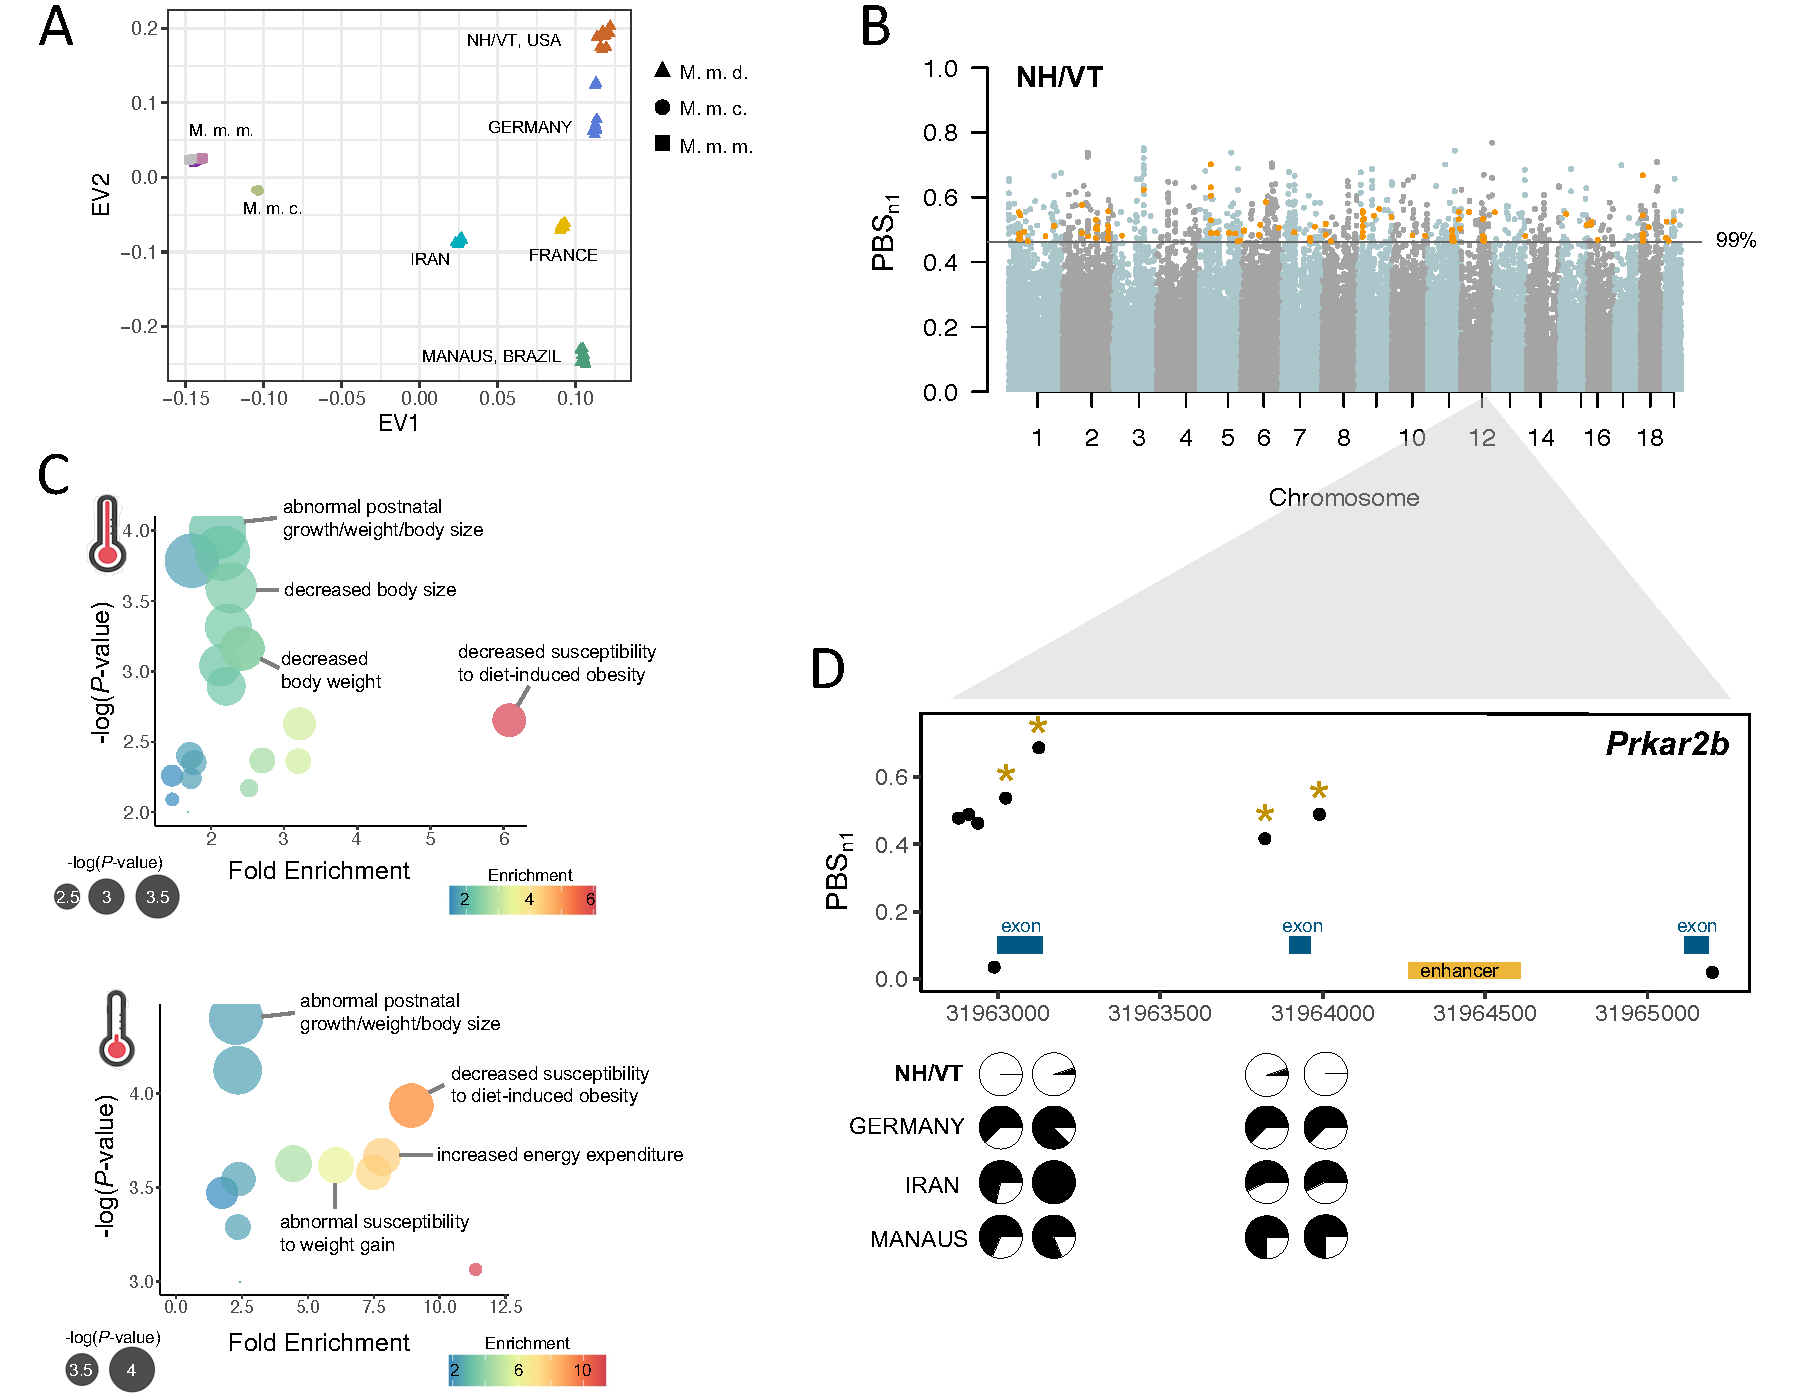
\includegraphics[width=\textwidth]{./figure_4_rev.pdf}
  \caption{\textbf{Genomic outliers are enriched in genes with evidence for} \textbf{\textit{cis}-regulatory divergence. (A)} Genetic PCA of wild house mice distinguished mouse populations based on population-of-origin (\textit{Mus musculus domesticus} (M.m.d.)) and subspecies (\textit{Mus musculus castaneus} (M.m.c.), \textit{Mus musculus musculus} (M.m.m.)). The x and y axes show the first and second SNP eigenvectors, respectively (EV; PC1: 29\% of variance, PC2: 8\% of variance. \textbf{(B)} Autosomal selection scan showing \textit{PBSn1} results for the New Hampshire/Vermont (NH/VT) focal population. Orange points depict genes that exhibit \textit{cis}-regulatory divergence and overlap with outlier regions. \textbf{(C)} Gene set enrichment analysis for genes with ASE that overlap genomic outliers in the NH/VT population. ASE outliers were highly enriched for mouse phenotypes related to body size differences and metabolic features, across both temperature treatments. \textbf{(D)} Candidate gene that exhibits \textit{cis}-regulatory divergence and overlaps with outlier region. Allele frequencies (pie charts) of significant SNPs (gold asterisks) in the four \textit{Mus musculus domesticus} populations.}
\end{figure*}

Next, to identify genetic signatures of adaptation in house mice from
the Americas, we performed a scan for regions of genetic differentiation
consistent with selection using a normalized version of the population
branch statistic. We used this test to identify highly differentiated
loci in our focal populations in the Americas (MAN and NH/VT) relative
to Eurasian populations (see Methods). In total, 83,538 and 84,420
non-overlapping 5-SNP windows were analyzed for MAN and NH/VT,
respectively. Outlier windows in NH/VT and MAN overlapped 538 and 530
genes, respectively (\emph{SI Appendix}, Dataset S1). Overall, genomic
outliers were distributed across the genome in both populations (Fig. 4B
and \emph{SI Appendix}, Fig. S12), consistent with selection acting
primarily on standing genetic variation in house mice (20, 21).

Finally, we asked to what extent genomic divergence among wild mice from
temperate and tropical environments is associated with
\emph{cis}-regulatory changes. Specifically, if natural selection
associated with climatic adaptation has acted mainly on regulatory
variants, we predicted an enrichment of genomic outliers near genes
exhibiting ASE (e.g., ref. 54). To test this prediction, we overlapped
putative candidate regions for selection based on SNP outlier windows
with genes for which we identified evidence for allele-specific
expression in BAT or liver. In NH/VT, we found outlier windows
overlapped 71 and 62 genes with evidence for \emph{cis}-regulatory
divergence under warm and cold conditions, respectively (overlap 44
genes) (Fig. 4B; \emph{SI Appendix}, Dataset S1). The overlap between
genes with \emph{cis}-regulatory divergence and outlier windows in this
population was greater than expected by chance (hypergeometric test,
\emph{P}=0.0016), and therefore is unlikely to be a consequence of
genetic drift. Moreover, genes with allele-specific expression were
associated with higher average population branch statistic scores than
background genes (\emph{P}=0.00026, see Methods). In contrast, we did
not find significant overlap between genes with allele-specific
expression and genomic outliers for Manaus (\emph{P}=0.4). Outlier
windows overlapped 49 and 51 genes with evidence for
\emph{cis}-regulatory divergence under warm and cold conditions,
respectively (\emph{SI Appendix}, Fig. S12). These genes were not
enriched for metabolic process terms or phenotypes.

Genes with allele-specific expression that overlapped genomic outliers
in temperate mice were enriched for mutant phenotypes related to body
size, growth, and metabolism relative to other genes with
\emph{cis}-regulatory divergence (e.g., abnormal postnatal
growth/weight/body size, abnormal susceptibility to weight gain,
decreased susceptibility to diet-induced obesity, and increased energy
expenditure; FDR \textless{} 0.05) (Fig. 4C; \emph{SI Appendix}, Dataset
S1). This gene set also includes genes whose expression in the liver was
previously associated with body mass variation in natural populations of
North American house mice (\emph{bcat2}, \emph{col6a1}, \emph{col5a2},
\emph{col3a1}) (21, 24). Additionally, this set included genes
implicated in obesity and metabolic phenotypes in humans (e.g.,
\emph{wrn}, \emph{plaat3}, \emph{prkar2b}, \emph{sulf2}, \emph{smoc1})
(Fig. 4D) (55) and mice (\emph{SI Appendix}, Table S4). Together, these
results suggest that selection has acted on \emph{cis}-regulatory genes
related to metabolism and body weight in North American mice (24).

\hypertarget{discussion}{%
\section*{Discussion}\label{discussion}}
\addcontentsline{toc}{section}{Discussion}

Understanding how both genetic and environmental factors influence gene
expression divergence is essential to understanding adaptive evolution.
Here, we utilized allele-specific expression in liver and brown adipose
tissue to characterize \emph{cis} and \emph{trans} changes underlying
expression differences between temperate and tropical house mice when
reared under warm and cold laboratory environments. We found that most
regulatory divergence was governed by \emph{cis}-regulatory variation,
and that these \emph{cis}-effects were largely independent of
environmental temperature. However, a subset of genes showed
temperature-dependent \emph{cis}-effects and thus represent QTL for
expression plasticity. Finally, overlap of genes exhibiting
\emph{cis}-regulatory divergence with scans for selection identified
several \emph{cis}-regulatory genes under positive selection, consistent
with a role for these loci in local adaptation. Together, our results
demonstrate how both genetic and environmental effects contribute to
adaptive gene expression differences between natural populations.

The rapid colonization of house mice into new environments may have been
mediated by plasticity through \emph{trans}-regulation. Specifically,
and similar to previous studies, we found that most expression
plasticity was largely governed by \emph{trans}-acting factors (43,
56--62), which modify correlated changes in gene expression profiles of
hundreds of genes. In fact, a large proportion of the correlated plastic
changes we observed went in the same direction as evolved expression
divergence, implicating a role for gene expression plasticity in the
colonization of new environments (22). Furthermore, this rapid response
via \emph{trans}-effects likely shifted to favor the predominant and
less pleiotropic \emph{cis}-regulatory architecture over time (62, 63).
We found that most \emph{cis}-effects were robust to temperature,
indicating a decoupling of environmental plasticity and allelic-effects.
Interestingly, a number of these \emph{cis}-regulatory loci show reduced
plasticity in temperate mice (\emph{SI Appendix}, Fig. S13), suggesting
that selection may target genetic changes that minimize plasticity (30,
32, 64).

Although most \emph{cis}-effects were robust to temperature, we
identified a subset of genes that showed temperature-dependent
\emph{cis}-effects. These loci are of particular interest since these
constitute \emph{plasticity}-eQTL and harbor mutations that directly
affect plasticity of gene expression. Genetic assimilation refers to the
conversion of a plastic response to a canalized response (65--68). If
the ancestral allele at a \emph{plasticity}-eQTL encodes a plastic
response and the derived allele encodes a canalized response, then the
\emph{plasticity}-eQTL represents a case of genetic assimilation. For
example, selection in a cold, temperate environment may have led to the
reduced plasticity exhibited in New York mice. A similar mechanism was
recently proposed by Verta \& Jones (2019) to explain the observed
plasticity in gene expression between freshwater and marine threespine
stickleback. \emph{Cis}-regulatory variants could rapidly canalize
expression through the loss or gain of specific binding sites for
conditionally expressed transcription factors, thereby decoupling a
gene's expression from the environment (69). Many of the \emph{cis} x
environment candidates illustrate potential regulatory mechanisms
underlying genetic assimilation as many of them exhibit reduced
plasticity in New York mice (\emph{SI Appendix}, Fig. S13). For example,
\emph{scd1} plays an important role in basal and cold-induced
thermogenesis (70, 71) and New York mice show higher and constitutive
average expression of \emph{scd1} in BAT compared to Brazil mice
(\emph{SI Appendix}, Fig. S13). Further study of these genes may help us
understand the relationship between plasticity, selection, and
adaptation to novel environments in natural populations.

Our comparison between New York and Brazil house mice across
environments has implications for our understanding of gene regulation
and genome function across short evolutionary timescales. Although house
mice colonized the Americas within the last \textasciitilde500 years, we
found evidence for pervasive \emph{cis}-regulatory divergence.
Furthermore, house mice have rapidly adapted to various environments
from pre-existing standing genetic variation (20, 21, 24, 72), which has
likely contributed to the predominance and enrichment of
\emph{cis}-regulatory variation associated with local adaptation in
temperate mice. We speculate that the significant overlap between
genomic outliers and ASE in temperate mice but not in tropical mice may
reflect adaptation predominantly to cold environments (rather than to
warm environments), consistent with the warm ancestral range of house
mice in the Mediterranean region. Nonetheless, positive selection may
preferentially act on \emph{cis}-acting alleles due to their higher
additivity and less sensitivity to genomic background (35, 62, 73).
Similarly, natural selection may target \emph{cis}-acting alleles due to
their insensitivity to environmental conditions, making them a primary
substrate for adaptation to novel environments (62). These features of
\emph{cis}-regulatory divergence allow them to accrue on extremely short
timescales, making them important loci for rapid climatic adaptation.

Overall, this study broadens our understanding of the role of gene
regulation in recent adaptive evolution by disentangling \emph{cis}- and
\emph{trans}-changes underlying genetic and environmental effects on
gene expression differences. While some progress has been made on the
relative importance of \emph{cis}- and \emph{trans}-changes in
adaptation within and between species (16, 36), most of the observed
differences in regulatory patterns have been measured in a single
environment, overlooking environment- and genotype-by-environment
effects. By pairing allele-specific expression across different
conditions with genomic data from natural populations, we discovered
important roles for environment-dependent \emph{trans}-changes and
environment-independent \emph{cis}-regulatory divergence in populations
adapting to new environments. Thus, this work provides insight into the
molecular architecture underlying genetic and non-genetic causes of gene
expression differences during adaptive evolution.

\hypertarget{materials-and-methods}{%
\section*{Materials and Methods}\label{materials-and-methods}}
\addcontentsline{toc}{section}{Materials and Methods}

\hypertarget{animals-and-evolved-phenotypic-differences}{%
\subsubsection*{Animals and Evolved Phenotypic
Differences}\label{animals-and-evolved-phenotypic-differences}}
\addcontentsline{toc}{subsubsection}{Animals and Evolved Phenotypic
Differences}

To characterize evolved phenotypic differences between New York and
Brazil house mice, we used two wild-derived inbred lines of house mice:
SARA (New York) and MANA (Brazil). Previous studies have demonstrated
that these lines vary in morphology and gene expression and are
indicative of population divergence (21, 23) (\emph{SI Appendix},
\emph{Supplementary Text}). The establishment of these lines has been
described previously (23). Mice from each line were housed in a standard
laboratory environment at 21\(^{\circ}\)C with a 12L:12D cycle. Roughly
equal numbers of males and females were produced for each within-line
comparison (\emph{n} = 32 per line; \emph{SI Appendix}, Dataset S1). We
took standard museum measurements on all mice and removed and prepared
dried skins. Thermal conductance of pelage (referred to as pelage
conductance {[}W m\textsuperscript{-2}
\textsuperscript{\(^{\circ}\)}C\textsuperscript{-1}{]}) was measured on
dry skins following the protocol of Riddell et al.~2022 (\emph{SI
Appendix, Supplementary Text}) (74). Tail length and ear length were
corrected for body mass for each individual. Effects of line and sex for
each phenotype were modeled using ANOVA. All statistical analyses were
performed using packages available in R (v.4.1.1).

\hypertarget{experimental-design-and-tissue-collection}{%
\subsubsection*{Experimental Design and Tissue
Collection}\label{experimental-design-and-tissue-collection}}
\addcontentsline{toc}{subsubsection}{Experimental Design and Tissue
Collection}

To investigate the gene regulatory mechanisms underlying local
adaptation in house mice, we generated F1 hybrids by crossing a SARA
female with a MANA male. All experimental animals were born at room
temperature (21\(^{\circ}\)C) and were provided water and commercial
rodent chow \emph{ad libitum}. We weaned and singly housed SARA, MANA,
and F1 hybrids at \textasciitilde3 weeks of age. We split 3.5-week-old
full-sibs and F1 hybrids into size-matched experimental groups across
cold (5\(^{\circ}\)C) and warm (21\(^{\circ}\)C) treatments. Mice were
kept in their respective experimental environment until
\textasciitilde12 weeks of age, at which point individuals were
euthanized via cervical dislocation. We took standard museum
measurements and then rapidly dissected and preserved liver and brown
adipose tissue in RNAlater at 4\(^{\circ}\)C overnight and moved to
-80\(^{\circ}\)C until RNA extraction. We prepared standard museum
skeletons and accessioned them in UC Berkeley's Museum of Vertebrate
Zoology (catalog numbers are given in \emph{SI Appendix}, Dataset S1).
All experimental procedures were in accordance with the UC Berkeley
Institutional Animal Care and Use Committee (AUP-2017-08-10248).

\hypertarget{rna-extraction-library-preparation-and-sequencing}{%
\subsubsection*{RNA Extraction, Library Preparation, and
Sequencing}\label{rna-extraction-library-preparation-and-sequencing}}
\addcontentsline{toc}{subsubsection}{RNA Extraction, Library
Preparation, and Sequencing}

We extracted total RNA from liver and BAT from each sample (\emph{n} =
\textasciitilde6 per genotype/sex/treatment/tissue) using the RNeasy
PowerLyzer Kit (QIAGEN). We generated Illumina cDNA libraries from 1
\(\mu\)g of purified RNA using KAPA Stranded mRNA-Seq Kit (Illumina),
and uniquely indexed libraries using unique dual indexes (Illumina).
Libraries were pooled in equal molar concentration and sequenced on one
lane each of 150 bp paired-end NovaSeq S1 and NovaSeq S4 at the Vincent
J. Coates Genomics Sequencing Center at UC Berkeley. We filtered raw
reads below a Phred quality score of 15 and trimmed adapter sequences
using \emph{fastp} (75).

\hypertarget{parental-gene-expression-analyses}{%
\subsubsection*{Parental Gene Expression
Analyses}\label{parental-gene-expression-analyses}}
\addcontentsline{toc}{subsubsection}{Parental Gene Expression Analyses}

After cleaning and trimming parental sequences of MANA and SARA, we
mapped reads to the \emph{Mus musculus} reference genome (GRCm38/mm10)
using STAR (76). We counted reads overlapping exons using HTSeq (77)
based on the Ensembl GRCm38.98 annotation. We imported raw count data
into R (v.4.1.1) and transformed expression values using variance
stabilizing transformation (78) to assess transcriptome-wide expression
patterns via PCA. Next, we removed genes with fewer than an average of
10 reads per individual within each tissue, retaining \textasciitilde14K
expressed genes per tissue for downstream analyses. We then used DESeq2
(78) on raw, filtered reads to quantify expression patterns by fitting a
generalized linear model following a negative binomial distribution
(Wald-test). Due to the strong effects of tissue-type and sex on
expression patterns (\emph{SI Appendix}, Fig. S1), we computed
differential expression between lines for each tissue and sex,
separately (but see \emph{SI Appendix}, \emph{Supplementary Text} for a
full parameterized model). Specifically, we used the model line +
environment + line*environment to determine the effects of genotype,
environment, and genotype-by-environment (GxE) on expression patterns.
We defined genes as GxE if: 1) only one genotype showed significant
differential expression between temperatures (``line-specific''), or 2)
both genotypes showed significant differences between temperatures, but
in opposite directions (``opposite''). Lastly, we used a
Benjamini-Hochberg multiple test correction (79) on all resulting
\textit{P}-values and considered genes with FDR \textless{} 0.05 to be
significantly differentially expressed.

To determine if gene expression plasticity is correlated with gene
expression divergence, we compared genes with significant plasticity in
Brazil mice to genes with significant expression divergence between
Brazil and New York mice within each tissue and sex, separately. We used
Spearman's rank correlation coefficients to assess overall
directionality and significance of gene expression. To account for
potential statistical artifacts in the regression (80), we compared the
observed correlations to a permuted distribution (10,000 permutations).

\hypertarget{identifying-variants-between-parental-lines}{%
\subsubsection*{Identifying Variants between Parental
Lines}\label{identifying-variants-between-parental-lines}}
\addcontentsline{toc}{subsubsection}{Identifying Variants between
Parental Lines}

To identify differences between lines for allele-specific read
assignment, we performed SNP calling on whole genome sequence data from
one female each of MANA and SARA. We mapped genomic reads with Bowtie2
(81) to the mm10 reference genome (setting: --very-sensitive) obtained
from Ensembl. We marked duplicates with the Picard tool MarkDuplicates
and then we used the GATK tools HaplotypeCaller and GenotypeGVCFs for
joint genotyping across genomic samples. We filtered for low quality SNP
calls with VariantFiltration (QD \textless{} 2.0; QUAL \textless{} 30.0;
FS \textgreater{} 200; ReadPosRankSum \textless{} -20.0). To reduce the
influence of genotyping error in whole genome sequencing data on
allele-specific expression assignment of RNA-seq reads (e.g., ref. 82),
we mapped RNA-seq reads from all individuals and then counted
allele-specific reads aligned to each site we genotyped with the GATK
tool ASEReadCounter. We excluded sites for which we did not have
coverage of at least 5 reads from each population-specific allele. In
total, 2,875,480 and 2,181,304 variants from MANA and SARA,
respectively, were used for identifying allele-specific reads.

\hypertarget{mapping-allele-specific-reads}{%
\subsubsection*{Mapping Allele-Specific
Reads}\label{mapping-allele-specific-reads}}
\addcontentsline{toc}{subsubsection}{Mapping Allele-Specific Reads}

For allele-specific expression analyses, we mapped reads from hybrid
individuals to the mouse reference genome (GRCm38/mm10) using STAR. We
used WASP (83) to reduce the potential for reference mapping bias.
Specifically, WASP mitigates mapping bias by identifying reads
containing SNPs, simulating reads with alternative alleles at that
locus, re-mapping these reads to the reference, and then flagging reads
that do not map to the same location. Reads that do not map to the same
location are then discarded. We retained reads that overlapped a
population-specific variant and that passed WASP filtering for our
allele-specific expression analysis. We separated reads overlapping
informative variants into allele-specific pools (NY, BZ) based on
genotype for quantification. We used HTSeq to count the number of reads
associated with each gene per population based on the overlap of reads
and annotated exonic regions based on the Ensembl GRCm38.98 annotation.
We examined per site allelic reads with ASEReadCounter to quantify
allele-specific mapping over individual sites. Proportions of reads
overlapping the references vs.~alternative allele (REF allele / (ALT
allele + REF allele)) showed a median 0.5 across samples (\emph{SI
Appendix}, Figs. S14-S15), indicating no evidence for reference mapping
bias.

\hypertarget{identifying-cis-and-trans-regulatory-divergene}{%
\subsubsection*{\texorpdfstring{Identifying \emph{Cis}- and
\emph{Trans}-Regulatory
Divergence}{Identifying Cis- and Trans-Regulatory Divergence}}\label{identifying-cis-and-trans-regulatory-divergene}}
\addcontentsline{toc}{subsubsection}{Identifying \emph{Cis}- and
\emph{Trans}-Regulatory Divergence}

Parental (F0) and F1 expression data was used to characterize \emph{cis}
and \emph{trans} effects. To categorize regulatory divergence at each
gene, we inferred differential expression by analyzing raw counts using
DESeq2. To identify genes with evidence of allele-specific expression in
hybrid individuals, we took reads that mapped preferentially to either
New York or Brazil alleles and fit these to a model with allele (NY
vs.~BZ), sample (individual), and tissue (BAT, liver) for hybrid male
samples in DESeq2 (Wald-test; \emph{SI Appendix}, \emph{Supplementary
Text}). As read counts come from the same sequencing library, library
size factor normalization was disabled in DESeq2 by setting SizeFactors
= 1 for measures of allele-specific expression. We used males to assign
regulatory categories to maximize power due to a larger number of hybrid
samples sequenced (6 replicates of males vs.~4 replicates of females),
though we also see similar regulatory patterns in females (\emph{SI
Appendix}, \emph{Supplementary Text} and Fig. S16). Differential
expression between alleles in the F1 is evidence for
\emph{cis}-regulatory divergence. Conversely, \emph{trans}-regulatory
divergence is inferred when differential expression in the F0 generation
is not recapitulated between alleles in the F1. The \emph{trans}
component (T) was assessed through a Fisher's Exact Test on reads
mapping to each parental allele in the hybrid vs.~parental read counts,
summed over all replicates (35, 84). We randomly down-sampled reads to
account for library size differences between parental and F1 replicates
(39, 85). \emph{P}-values for each test were corrected for FDR with the
Benjamini-Hochberg method. We sorted genes into categories based on an
FDR threshold of 5\% (35, 84), as described below. We analyzed
temperature treatments (warm and cold) separately for regulatory
assignment and then compared as described below:\\
\indent \textit{Conserved}: no significant difference between lines
(F0), no significant difference between alleles (F1), no significant
\textit{T}.\\
\indent \textit{Cis} only: significant difference between lines (F0),
significant difference between alleles (F1), no significant
\textit{T}.\\
\indent \textit{Trans} only: significant difference between lines (F0),
no significant difference between alleles (F1), significant
\textit{T}.\\
\indent \emph{Cis} {\&} \emph{Trans} designations: significant
differences between alleles (F1) and significant \textit{T}. This
category was further subdivided into \emph{cis} + \emph{trans}
(reinforcing), \emph{cis} + \emph{trans} (opposing),
\textit{compensatory}, and \emph{cis} x \emph{trans}, as previously
described (37, 39).\\
\indent \emph{Ambiguous}: all other patterns.

We identified \emph{cis} x temperature interactions using DESeq2 under a
model specifying temperature (cold vs.~warm) and allele (BZ vs.~NY). To
identify \emph{trans} x temperature interactions, we fit a model that
included parental and hybrid read counts for temperature (cold
vs.~warm), allele/genotype (BZ vs.~NY), and generation (F1 vs.~F0) and
interactions. We considered genes significant at an FDR threshold of
10\%, consistent with previous studies (e.g., refs. 62, 86) as our
statistical analysis has less power to detect interactions than main
effects. Similar models were also used to identify sex- and
tissue-specific regulatory patterns in DESeq2 (\emph{SI Appendix},
\emph{Supplementary Text}).

\hypertarget{genetic-PCA-of-M.m-domesticus-populations}{%
\subsubsection*{\texorpdfstring{Genetic PCA of \emph{M.m.domesticus}
populations}{Genetic PCA of M.m.domesticus populations}}\label{genetic-PCA-of-M.m-domesticus-populations}}
\addcontentsline{toc}{subsubsection}{Genetic PCA of
\emph{M.m.domesticus} populations}

We used SNPRelate (87) to perform PCA and IBS hierarchical clustering of
population genetic data. Genomic data from 3 Eurasian populations of
\emph{M. m. domesticus} (Germany {[}Cologne-Bonn{]}, France, and Iran)
and \emph{M. m. musculus} and \emph{M. m. castaneus} subspecies were
downloaded from \url{http://wwwuser.gwdg.de/~evolbio/evolgen/wildmouse/}
(50). For PCA, biallelic variants genotyped across all these individuals
were extracted and pruned for linkage disequilibrium in SNPRelate
(thresholds=0.2) resulting in 22,126 variant sites for PCA and IBS
clustering for \emph{M. m. domesticus} comparisons and 25,467 variants
for global \emph{Mus} comparisons (Fig. 4A and \emph{SI Appendix}, Fig.
S11). Altering the pruning threshold to 0.5 did not result in any change
in population clustering.

\hypertarget{autosomal-scans-for-selection}{%
\subsubsection*{Autosomal Scans for
Selection}\label{autosomal-scans-for-selection}}
\addcontentsline{toc}{subsubsection}{Autosomal Scans for Selection}

To identify regions with evidence for selection in the Americas, we
scanned the exomes of our North and South American focal populations for
selection by using a modification of the population branch statistic
(PBS) which summarizes a three-way comparison of allele frequencies
between a focal group, a closely related population, and an outgroup
comparison (\emph{PBSn1}) (88, 89):
\[ PBSn1 = {PBS_1 \over 1 + PBS_1 + PBS_2 + PBS_3}  \]

Here, \emph{PBS1} indicates PBS calculated as either Manaus or NH/VT as
the focal population, and \emph{PBS2} and \emph{PBS3} indicate PBS
calculated for Eurasians populations as the focal populations (France or
Germany and Iran, respectively). To maximize the number of sites that
could be compared, American populations are not directly compared in the
branch test due to the reduced representation of exome data and high per
site Fst values between the two populations (\emph{SI Appendix}, Fig.
S17). Instead, NH/VT and MAN were each compared to two Eurasian
populations {[}((MAN), France) Iran) and ((NH/VT) Germany) Iran){]},
selected based on population clustering (\emph{SI Appendix}, Fig. S11).
We restricted our SNP set to biallelic variants across the 3 populations
being compared and required that at least six individuals in the focal
branch be genotyped. We note that the NH/VT sample used in the PBS test
is geographically close to the origin of the SARA line.

We used VCFtools (90) to calculate Weir and Cockerham Fst at each
variant position. These values were used to calculate \emph{PBSn1} for
non-overlapping blocks of 5 SNPs. We consider blocks in the top 1\% of
\emph{PBSn1} scores outliers and do not attempt to assign
\emph{P}-values to each SNP-block (91). Genomic outliers were
\textgreater3 standard deviations above the mean windowed value of
SNP-blocks in each comparison (MAN focal, median=0.045; NH/VT focal
median = 0.064). We refer to these genes as ``genomic outliers'' given
the selection scan did not consider neutral models of evolution. We
identified windows overlapping genes based on Ensembl gene coordinates
(mm10) and the BEDTools ``intersect'' tool (92). As allele-specific
expression in F1s is consistent with local independent genetic changes
influencing gene expression, we focused on genes with evidence for
\emph{cis}-regulatory divergence (i.e., differences in expression
between parental alleles in the F1) for overlap with outlier loci. To
ask whether allele-specific expression was associated with elevated
\emph{PBSn1} scores, we used a generalized linear model incorporating
gene category (ASE or no ASE) and SNP density per kb as factors to
\emph{PBSn1} scores. SNP density was calculated by dividing the number
of informative sites between NY and BZ for allele-specific expression
per gene by transcript length.

\hypertarget{enrichment-analyses}{%
\subsubsection*{Enrichment Analyses}\label{enrichment-analyses}}
\addcontentsline{toc}{subsubsection}{Enrichment Analyses}

We performed all GO and pathway enrichment analyses with PANTHER (93,
94). For GO enrichment associated with \emph{cis}-regulatory divergence,
we defined the background set of genes as all \emph{cis}-regulated genes
tested within a tissue. We performed phenotype enrichment analyses with
ModPhea (95), and we annotated genes to specific phenotypes based on
Mouse Genome Informatics phenotype annotations
(\url{http://www.informatics.jax.org/}).

\hypertarget{data-availability}{%
\subsubsection*{Data Availability}\label{data-availability}}
\addcontentsline{toc}{subsubsection}{Data Availability}

Scripts are available on
GitHub(\url{https://github.com/malballinger/BallingerMack_NYBZase_2023}),with
the repository archived in Zenodo (accession pending). All sequence data
generated in this study have been deposited to the National Center for
Biotechnology Information Sequence Read Archive under accession
BioProject ID PRJNAXXX. All other data are included in the article
and/or \emph{SI Appendix}.

\showmatmethods
\showacknow
\pnasbreak

\hypertarget{references}{%
\section*{References}\label{references}}
\addcontentsline{toc}{section}{References}

\hypertarget{refs}{}
\begin{CSLReferences}{0}{0}
\leavevmode\vadjust pre{\hypertarget{ref-King1975}{}}%
\CSLLeftMargin{1. }%
\CSLRightInline{King MC, Wilson AC (1975) Evolution at two levels in
humans and chimpanzees. \emph{Science} 188(4184):107--116.}

\leavevmode\vadjust pre{\hypertarget{ref-Wray2003}{}}%
\CSLLeftMargin{2. }%
\CSLRightInline{Wray GA, et al. (2003) The evolution of transcriptional
regulation in eukaryotes. \emph{Mol Biol Evol} 20(9):1377--1419.}

\leavevmode\vadjust pre{\hypertarget{ref-Jones2012}{}}%
\CSLLeftMargin{3. }%
\CSLRightInline{Jones FC, et al. (2012) The genomic basis of adaptive
evolution in threespine sticklebacks. \emph{Nature} 484(7392):55--61.}

\leavevmode\vadjust pre{\hypertarget{ref-Fraser2013}{}}%
\CSLLeftMargin{4. }%
\CSLRightInline{Fraser HB (2013) Gene expression drives local adaptation
in humans. \emph{Genome Res} 23(7):1089--1096.}

\leavevmode\vadjust pre{\hypertarget{ref-Gibson2008}{}}%
\CSLLeftMargin{5. }%
\CSLRightInline{Gibson G (2008) The environmental contribution to gene
expression profiles. \emph{Nat Rev Genet} 9(8):575--581.}

\leavevmode\vadjust pre{\hypertarget{ref-Grishkevich2013}{}}%
\CSLLeftMargin{6. }%
\CSLRightInline{Grishkevich V, Yanai I (2013) The genomic determinants
of genotype\(\times\) environment interactions in gene expression.
\emph{Trends in Genetics} 29(8):479--487.}

\leavevmode\vadjust pre{\hypertarget{ref-Hodgins2009}{}}%
\CSLLeftMargin{7. }%
\CSLRightInline{Hodgins-Davis A, Townsend JP (2009) Evolving gene
expression: From g to e to g\(\times\) e. \emph{Trends Ecol Evol}
24(12):649--658.}

\leavevmode\vadjust pre{\hypertarget{ref-Lopez2008}{}}%
\CSLLeftMargin{8. }%
\CSLRightInline{López-Maury L, Marguerat S, Bähler J (2008) Tuning gene
expression to changing environments: From rapid responses to
evolutionary adaptation. \emph{Nat Rev Genet} 9(8):583--593.}

\leavevmode\vadjust pre{\hypertarget{ref-West-Eberhard2003}{}}%
\CSLLeftMargin{9. }%
\CSLRightInline{West-Eberhard MJ (2003) \emph{Developmental plasticity
and evolution} (Oxford University Press).}

\leavevmode\vadjust pre{\hypertarget{ref-Ghalambor2007}{}}%
\CSLLeftMargin{10. }%
\CSLRightInline{Ghalambor CK, McKay JK, Carroll SP, Reznick DN (2007)
Adaptive versus non-adaptive phenotypic plasticity and the potential for
contemporary adaptation in new environments. \emph{Funct Ecol}
21(3):394--407.}

\leavevmode\vadjust pre{\hypertarget{ref-Corl2018}{}}%
\CSLLeftMargin{11. }%
\CSLRightInline{Corl A, et al. (2018) The genetic basis of adaptation
following plastic changes in coloration in a novel environment.
\emph{Curr Biol} 28(18):2970--2977.e7.}

\leavevmode\vadjust pre{\hypertarget{ref-Wray2007}{}}%
\CSLLeftMargin{12. }%
\CSLRightInline{Wray GA (2007) The evolutionary significance of
\emph{cis}-regulatory mutations. \emph{Nat Rev Genet} 8(3):206--216.}

\leavevmode\vadjust pre{\hypertarget{ref-Wittkopp2011}{}}%
\CSLLeftMargin{13. }%
\CSLRightInline{Wittkopp PJ, Kalay G (2011) \emph{Cis}-regulatory
elements: Molecular mechanisms and evolutionary processes underlying
divergence. \emph{Nat Rev Genet} 13(1):59--69.}

\leavevmode\vadjust pre{\hypertarget{ref-Carroll2008}{}}%
\CSLLeftMargin{14. }%
\CSLRightInline{Carroll SB (2008) Evo-devo and an expanding evolutionary
synthesis: A genetic theory of morphological evolution. \emph{Cell}
134(1):25--36.}

\leavevmode\vadjust pre{\hypertarget{ref-Stern2008}{}}%
\CSLLeftMargin{15. }%
\CSLRightInline{Stern DL, Orgogozo V (2008) The loci of evolution: How
predictable is genetic evolution? \emph{Evolution} 62(9):2155--2177.}

\leavevmode\vadjust pre{\hypertarget{ref-Signor2018}{}}%
\CSLLeftMargin{16. }%
\CSLRightInline{Signor SA, Nuzhdin SV (2018) The evolution of gene
expression in \emph{cis} and \emph{trans}. \emph{Trends Genet}
34(7):532--544.}

\leavevmode\vadjust pre{\hypertarget{ref-Cooper2003}{}}%
\CSLLeftMargin{17. }%
\CSLRightInline{Cooper TF, Rozen DE, Lenski RE (2003) Parallel changes
in gene expression after 20,000 generations of evolution in
\emph{escherichia coli}. \emph{Proc Natl Acad Sci} 100(3):1072--1077.}

\leavevmode\vadjust pre{\hypertarget{ref-Stern2009}{}}%
\CSLLeftMargin{18. }%
\CSLRightInline{Stern DL, Orgogozo V (2009) Is genetic evolution
predictable? \emph{Science} 323(5915):746--751.}

\leavevmode\vadjust pre{\hypertarget{ref-Lynch1992}{}}%
\CSLLeftMargin{19. }%
\CSLRightInline{Lynch CB (1992) Clinal variation in cold adaptation in
\emph{mus} \emph{domesticus}: Verification of predictions from
laboratory populations. \emph{Am Nat} 139(6):1219--1236.}

\leavevmode\vadjust pre{\hypertarget{ref-Ferris2021}{}}%
\CSLLeftMargin{20. }%
\CSLRightInline{Ferris KG, et al. (2021) The genomics of rapid climatic
adaptation and parallel evolution in {North American} house mice.
\emph{PLoS Genet} 17(4):e1009495.}

\leavevmode\vadjust pre{\hypertarget{ref-Phifer-Rixey2018}{}}%
\CSLLeftMargin{21. }%
\CSLRightInline{Phifer-Rixey M, et al. (2018) The genomic basis of
environmental adaptation in house mice. \emph{PLoS Genet}
14(9):e1007672.}

\leavevmode\vadjust pre{\hypertarget{ref-Bittner2021}{}}%
\CSLLeftMargin{22. }%
\CSLRightInline{Bittner NKJ, Mack KL, Nachman MW (2021) Gene expression
plasticity and desert adaptation in house mice. \emph{Evolution}
75(6):1477--1491.}

\leavevmode\vadjust pre{\hypertarget{ref-Ballinger2022}{}}%
\CSLLeftMargin{23. }%
\CSLRightInline{Ballinger MA, Nachman MW (2022) The contribution of
genetic and environmental effects to {Bergmann's} rule and {Allen's}
rule in house mice. \emph{Am Nat} 199(5):691--704.}

\leavevmode\vadjust pre{\hypertarget{ref-Mack2018}{}}%
\CSLLeftMargin{24. }%
\CSLRightInline{Mack KL, Ballinger MA, Phifer-Rixey M, Nachman MW (2018)
Gene regulation underlies environmental adaptation in house mice.
\emph{Genome Res} 28(11):1636--1645.}

\leavevmode\vadjust pre{\hypertarget{ref-Abumrad2017}{}}%
\CSLLeftMargin{25. }%
\CSLRightInline{Abumrad NA (2017) The liver as a hub in thermogenesis.
\emph{Cell Metab} 26(3):454--455.}

\leavevmode\vadjust pre{\hypertarget{ref-Simcox2017}{}}%
\CSLLeftMargin{26. }%
\CSLRightInline{Simcox J, et al. (2017) Global analysis of plasma lipids
identifies {liver-derived} acylcarnitines as a fuel source for brown fat
thermogenesis. \emph{Cell Metab} 26(3):509--522.e6.}

\leavevmode\vadjust pre{\hypertarget{ref-Cannon2004}{}}%
\CSLLeftMargin{27. }%
\CSLRightInline{Cannon B, Nedergaard J (2004) Brown adipose tissue:
Function and physiological significance. \emph{Physiol Rev}
84(1):277--359.}

\leavevmode\vadjust pre{\hypertarget{ref-Price2003}{}}%
\CSLLeftMargin{28. }%
\CSLRightInline{Price TD, Qvarnström A, Irwin DE (2003) The role of
phenotypic plasticity in driving genetic evolution. \emph{Proc Biol Sci}
270(1523):1433--1440.}

\leavevmode\vadjust pre{\hypertarget{ref-Ghalambor2015}{}}%
\CSLLeftMargin{29. }%
\CSLRightInline{Ghalambor CK, et al. (2015) Non-adaptive plasticity
potentiates rapid adaptive evolution of gene expression in nature.
\emph{Nature} 525(7569):372--375.}

\leavevmode\vadjust pre{\hypertarget{ref-Fischer2016}{}}%
\CSLLeftMargin{30. }%
\CSLRightInline{Fischer EK, Ghalambor CK, Hoke KL (2016) Can a network
approach resolve how adaptive vs nonadaptive plasticity impacts
evolutionary trajectories? \emph{Integr Comp Biol} 56(5):877--888.}

\leavevmode\vadjust pre{\hypertarget{ref-Josephs2021}{}}%
\CSLLeftMargin{31. }%
\CSLRightInline{Josephs EB, Van Etten ML, Harkess A, Platts A, Baucom RS
(2021) Adaptive and maladaptive expression plasticity underlying
herbicide resistance in an agricultural weed. \emph{Evol Lett}
5(4):432--440.}

\leavevmode\vadjust pre{\hypertarget{ref-Campbell2021}{}}%
\CSLLeftMargin{32. }%
\CSLRightInline{Campbell-Staton SC, Velotta JP, Winchell KM (2021)
Selection on adaptive and maladaptive gene expression plasticity during
thermal adaptation to urban heat islands. \emph{Nat Commun} 12(1):6195.}

\leavevmode\vadjust pre{\hypertarget{ref-Cowles2002}{}}%
\CSLLeftMargin{33. }%
\CSLRightInline{Cowles CR, Hirschhorn JN, Altshuler D, Lander ES (2002)
Detection of regulatory variation in mouse genes. \emph{Nat Genet}
32(3):432--437.}

\leavevmode\vadjust pre{\hypertarget{ref-Wittkopp2004}{}}%
\CSLLeftMargin{34. }%
\CSLRightInline{Wittkopp PJ, Haerum BK, Clark AG (2004) Evolutionary
changes in \emph{cis} and \emph{trans} gene regulation. \emph{Nature}
430(6995):85--88.}

\leavevmode\vadjust pre{\hypertarget{ref-McManus2010}{}}%
\CSLLeftMargin{35. }%
\CSLRightInline{McManus CJ, et al. (2010) Regulatory divergence in
drosophila revealed by {mRNA-seq}. \emph{Genome Res} 20(6):816--825.}

\leavevmode\vadjust pre{\hypertarget{ref-Hill2021}{}}%
\CSLLeftMargin{36. }%
\CSLRightInline{Hill MS, Vande Zande P, Wittkopp PJ (2021) Molecular and
evolutionary processes generating variation in gene expression.
\emph{Nat Rev Genet} 22(4):203--215.}

\leavevmode\vadjust pre{\hypertarget{ref-Goncalves2012}{}}%
\CSLLeftMargin{37. }%
\CSLRightInline{Goncalves A, et al. (2012) Extensive compensatory
cis-trans regulation in the evolution of mouse gene expression.
\emph{Genome Res} 22(12):2376--2384.}

\leavevmode\vadjust pre{\hypertarget{ref-Shen2014}{}}%
\CSLLeftMargin{38. }%
\CSLRightInline{Shen SQ, Turro E, Corbo JC (2014) Hybrid mice reveal
parent-of-origin and \emph{cis}- and \emph{trans}-regulatory effects in
the retina. \emph{PLoS One} 9(10):e109382.}

\leavevmode\vadjust pre{\hypertarget{ref-Mack2016}{}}%
\CSLLeftMargin{39. }%
\CSLRightInline{Mack KL, Campbell P, Nachman MW (2016) Gene regulation
and speciation in house mice. \emph{Genome Res} 26(4):451--461.}

\leavevmode\vadjust pre{\hypertarget{ref-Crowley2015}{}}%
\CSLLeftMargin{40. }%
\CSLRightInline{Crowley JJ, et al. (2015) Analyses of allele-specific
gene expression in highly divergent mouse crosses identifies pervasive
allelic imbalance. \emph{Nat Genet} 47(4):353--360.}

\leavevmode\vadjust pre{\hypertarget{ref-Van2018}{}}%
\CSLLeftMargin{41. }%
\CSLRightInline{Gestel J van, Weissing FJ (2018) Is plasticity caused by
single genes? \emph{Nature} 555(7698):E19--E20.}

\leavevmode\vadjust pre{\hypertarget{ref-He2021}{}}%
\CSLLeftMargin{42. }%
\CSLRightInline{He F, et al. (2021) \emph{Cis}-regulatory evolution
spotlights species differences in the adaptive potential of gene
expression plasticity. \emph{Nat Commun} 12(1):3376.}

\leavevmode\vadjust pre{\hypertarget{ref-Li2006}{}}%
\CSLLeftMargin{43. }%
\CSLRightInline{Li Y, et al. (2006) Mapping determinants of gene
expression plasticity by genetical genomics in c. elegans. \emph{PLoS
Genet} 2(12):e222.}

\leavevmode\vadjust pre{\hypertarget{ref-Fumagalli2015}{}}%
\CSLLeftMargin{44. }%
\CSLRightInline{Fumagalli M, et al. (2015) Greenlandic inuit show
genetic signatures of diet and climate adaptation. \emph{Science}
349(6254):1343--1347.}

\leavevmode\vadjust pre{\hypertarget{ref-Hallmark2019}{}}%
\CSLLeftMargin{45. }%
\CSLRightInline{Hallmark B, et al. (2019) Genomic evidence of local
adaptation to climate and diet in indigenous siberians. \emph{Mol Biol
Evol} 36(2):315--327.}

\leavevmode\vadjust pre{\hypertarget{ref-Shore2013}{}}%
\CSLLeftMargin{46. }%
\CSLRightInline{Shore AM, et al. (2013) Cold-induced changes in gene
expression in brown adipose tissue, white adipose tissue and liver.
\emph{PLoS One} 8(7):e68933.}

\leavevmode\vadjust pre{\hypertarget{ref-Westerberg2006}{}}%
\CSLLeftMargin{47. }%
\CSLRightInline{Westerberg R, et al. (2006) {ELOVL3} is an important
component for early onset of lipid recruitment in brown adipose tissue*.
\emph{J Biol Chem} 281(8):4958--4968.}

\leavevmode\vadjust pre{\hypertarget{ref-Fraser2010}{}}%
\CSLLeftMargin{48. }%
\CSLRightInline{Fraser HB, Moses AM, Schadt EE (2010) Evidence for
widespread adaptive evolution of gene expression in budding yeast.
\emph{Proc Natl Acad Sci U S A} 107(7):2977--2982.}

\leavevmode\vadjust pre{\hypertarget{ref-Fraser2011}{}}%
\CSLLeftMargin{49. }%
\CSLRightInline{Fraser HB, et al. (2011) Systematic detection of
polygenic cis-regulatory evolution. \emph{PLoS Genet} 7(3):e1002023.}

\leavevmode\vadjust pre{\hypertarget{ref-Harr2016}{}}%
\CSLLeftMargin{50. }%
\CSLRightInline{Harr B, et al. (2016) Genomic resources for wild
populations of the house mouse, \emph{mus musculus} and its close
relative \emph{mus spretus}. \emph{Sci Data} 3(1):1--14.}

\leavevmode\vadjust pre{\hypertarget{ref-Tichy1994}{}}%
\CSLLeftMargin{51. }%
\CSLRightInline{Tichy H, Zaleska-Rutczynska Z, O'Huigin C, Figueroa F,
Klein J (1994) Origin of the north american house mouse. \emph{Folia
Biol} 40(6):483--496.}

\leavevmode\vadjust pre{\hypertarget{ref-Morgan2022}{}}%
\CSLLeftMargin{52. }%
\CSLRightInline{Morgan AP, et al. (2022) Population structure and
inbreeding in wild house mice (mus musculus) at different geographic
scales. \emph{Heredity} 129(3):183--194.}

\leavevmode\vadjust pre{\hypertarget{ref-Agwamba2023}{}}%
\CSLLeftMargin{53. }%
\CSLRightInline{Agwamba KD, Nachman MW (2023) The demographic history of
house mice (mus musculus domesticus) in eastern north america. \emph{G3}
13(2).}

\leavevmode\vadjust pre{\hypertarget{ref-York2018}{}}%
\CSLLeftMargin{54. }%
\CSLRightInline{York RA, et al. (2018) Behavior-dependent \emph{cis}
regulation reveals genes and pathways associated with bower building in
cichlid fishes. \emph{Proc Natl Acad Sci} 115(47):E11081--E11090.}

\leavevmode\vadjust pre{\hypertarget{ref-Berube2013}{}}%
\CSLLeftMargin{55. }%
\CSLRightInline{Bérubé J, Garand C, Lettre G, Lebel M (2013) The
non-synonymous polymorphism at position 114 of the {WRN} protein affects
cholesterol efflux in vitro and correlates with cholesterol levels in
vivo. \emph{Exp Gerontol} 48(6):533--538.}

\leavevmode\vadjust pre{\hypertarget{ref-Chen2015}{}}%
\CSLLeftMargin{56. }%
\CSLRightInline{Chen J, Nolte V, Schlötterer C (2015) Temperature stress
mediates decanalization and dominance of gene expression in drosophila
melanogaster. \emph{PLoS Genet} 11(2):e1004883.}

\leavevmode\vadjust pre{\hypertarget{ref-Ding2022}{}}%
\CSLLeftMargin{57. }%
\CSLRightInline{Ding SD, et al. (2022) Trans-regulatory changes underpin
the evolution of the drosophila immune response. \emph{PLoS Genetics}
18(11):e1010453.}

\leavevmode\vadjust pre{\hypertarget{ref-Li2017}{}}%
\CSLLeftMargin{58. }%
\CSLRightInline{Li XC, Fay JC (2017) {Cis-regulatory} divergence in gene
expression between two thermally divergent yeast species. \emph{Genome
Biol Evol} 9(5):1120--1129.}

\leavevmode\vadjust pre{\hypertarget{ref-Promislow2005}{}}%
\CSLLeftMargin{59. }%
\CSLRightInline{Promislow D (2005) A regulatory network analysis of
phenotypic plasticity in yeast. \emph{Am Nat} 165(5):515--523.}

\leavevmode\vadjust pre{\hypertarget{ref-Smith2008}{}}%
\CSLLeftMargin{60. }%
\CSLRightInline{Smith EN, Kruglyak L (2008) Gene-environment interaction
in yeast gene expression. \emph{PLoS Biol} 6(4):e83.}

\leavevmode\vadjust pre{\hypertarget{ref-Tirosh2009}{}}%
\CSLLeftMargin{61. }%
\CSLRightInline{Tirosh I, Reikhav S, Levy AA, Barkai N (2009) A yeast
hybrid provides insight into the evolution of gene expression
regulation. \emph{Science} 324(5927):659--662.}

\leavevmode\vadjust pre{\hypertarget{ref-Verta2019}{}}%
\CSLLeftMargin{62. }%
\CSLRightInline{Verta J-P, Jones FC (2019) Predominance of
\emph{cis}-regulatory changes in parallel expression divergence of
sticklebacks. \emph{eLife} 8:e43785.}

\leavevmode\vadjust pre{\hypertarget{ref-Vande2022}{}}%
\CSLLeftMargin{63. }%
\CSLRightInline{Vande Zande P, Wittkopp PJ (2022) Network topology can
explain differences in pleiotropy between cis-and trans-regulatory
mutations. \emph{Mol Biol Evol} 39(12):msac266.}

\leavevmode\vadjust pre{\hypertarget{ref-Ho2018}{}}%
\CSLLeftMargin{64. }%
\CSLRightInline{Ho W-C, Zhang J (2018) Evolutionary adaptations to new
environments generally reverse plastic phenotypic changes. \emph{Nat
Commun} 9(1):350.}

\leavevmode\vadjust pre{\hypertarget{ref-Waddington1942}{}}%
\CSLLeftMargin{65. }%
\CSLRightInline{Waddington CH (1942) Canalization of development and the
inheritance of acquired characters. \emph{Nature} 150(3811):563--565.}

\leavevmode\vadjust pre{\hypertarget{ref-Waddington1952}{}}%
\CSLLeftMargin{66. }%
\CSLRightInline{Waddington CH (1952) Selection of the genetic basis for
an acquired character. \emph{Nature} 169(4302):625--626.}

\leavevmode\vadjust pre{\hypertarget{ref-Waddington1953}{}}%
\CSLLeftMargin{67. }%
\CSLRightInline{Waddington CH (1953) Genetic assimilation of an acquired
character. \emph{Evolution} 7(2):118--126.}

\leavevmode\vadjust pre{\hypertarget{ref-Van_der_Burg2020}{}}%
\CSLLeftMargin{68. }%
\CSLRightInline{Burg KRL van der, et al. (2020) Genomic architecture of
a genetically assimilated seasonal color pattern. \emph{Science}
370(6517):721--725.}

\leavevmode\vadjust pre{\hypertarget{ref-Ehrenreich2016}{}}%
\CSLLeftMargin{69. }%
\CSLRightInline{Ehrenreich IM, Pfennig DW (2016) Genetic assimilation: A
review of its potential proximate causes and evolutionary consequences.
\emph{Ann Bot} 117(5):769--779.}

\leavevmode\vadjust pre{\hypertarget{ref-Ntambi2002}{}}%
\CSLLeftMargin{70. }%
\CSLRightInline{Ntambi JM, et al. (2002) Loss of {stearoyl-CoA}
desaturase-1 function protects mice against adiposity. \emph{Proc Natl
Acad Sci} 99(17):11482--11486.}

\leavevmode\vadjust pre{\hypertarget{ref-Lee2004}{}}%
\CSLLeftMargin{71. }%
\CSLRightInline{Lee S-H, et al. (2004) Lack of {stearoyl-CoA} desaturase
1 upregulates basal thermogenesis but causes hypothermia in a cold
environment. \emph{J Lipid Res} 45(9):1674--1682.}

\leavevmode\vadjust pre{\hypertarget{ref-Beckman2022}{}}%
\CSLLeftMargin{72. }%
\CSLRightInline{Beckman EJ, et al. (2022) The genomic basis of
high-elevation adaptation in wild house mice (mus musculus domesticus)
from south america. \emph{Genetics} 220(2):iyab226.}

\leavevmode\vadjust pre{\hypertarget{ref-Lemos2008}{}}%
\CSLLeftMargin{73. }%
\CSLRightInline{Lemos B, Araripe LO, Fontanillas P, Hartl DL (2008)
Dominance and the evolutionary accumulation of \emph{cis}- and
\emph{trans}-effects on gene expression. \emph{Proc Natl Acad Sci U S A}
105(38):14471--14476.}

\leavevmode\vadjust pre{\hypertarget{ref-Riddell2022}{}}%
\CSLLeftMargin{74. }%
\CSLRightInline{Riddell EA, Patton JL, Beissinger SR (2022) Thermal
adaptation of pelage in desert rodents balances cooling and insulation.
\emph{Evolution} 76(12):3001--3013.}

\leavevmode\vadjust pre{\hypertarget{ref-Chen2018}{}}%
\CSLLeftMargin{75. }%
\CSLRightInline{Chen S, Zhou Y, Chen Y, Gu J (2018) Fastp: An ultra-fast
all-in-one {FASTQ} preprocessor. \emph{Bioinformatics}
34(17):i884--i890.}

\leavevmode\vadjust pre{\hypertarget{ref-Dobin2013}{}}%
\CSLLeftMargin{76. }%
\CSLRightInline{Dobin A, et al. (2013) {STAR}: Ultrafast universal
{RNA-seq} aligner. \emph{Bioinformatics} 29(1):15--21.}

\leavevmode\vadjust pre{\hypertarget{ref-Anders2015}{}}%
\CSLLeftMargin{77. }%
\CSLRightInline{Anders S, Pyl PT, Huber W (2015) {HTSeq--a} python
framework to work with high-throughput sequencing data.
\emph{Bioinformatics} 31(2):166--169.}

\leavevmode\vadjust pre{\hypertarget{ref-Love2014}{}}%
\CSLLeftMargin{78. }%
\CSLRightInline{Love MI, Huber W, Anders S (2014) Moderated estimation
of fold change and dispersion for {RNA-seq} data with {DESeq2}.
\emph{Genome Biol} 15(12):550.}

\leavevmode\vadjust pre{\hypertarget{ref-Benjamini1995}{}}%
\CSLLeftMargin{79. }%
\CSLRightInline{Benjamini Y, Hochberg Y (1995) Controlling the false
discovery rate: A practical and powerful approach to multiple testing.
\emph{J R Stat Soc Series B Stat Methodol} 57(1):289--300.}

\leavevmode\vadjust pre{\hypertarget{ref-Mallard2018}{}}%
\CSLLeftMargin{80. }%
\CSLRightInline{Mallard F, Jakšić AM, Schlötterer C (2018) Contesting
the evidence for non-adaptive plasticity. \emph{Nature}
555(7698):E21--E22.}

\leavevmode\vadjust pre{\hypertarget{ref-Langmead2012}{}}%
\CSLLeftMargin{81. }%
\CSLRightInline{Langmead B, Salzberg SL (2012) Fast gapped-read
alignment with bowtie 2. \emph{Nat Methods} 9(4):357--359.}

\leavevmode\vadjust pre{\hypertarget{ref-Fresard2019}{}}%
\CSLLeftMargin{82. }%
\CSLRightInline{Frésard L, et al. (2019) Identification of rare-disease
genes using blood transcriptome sequencing and large control cohorts.
\emph{Nature medicine} 25(6):911--919.}

\leavevmode\vadjust pre{\hypertarget{ref-Van_de_Geijn2015}{}}%
\CSLLeftMargin{83. }%
\CSLRightInline{Geijn B van de, McVicker G, Gilad Y, Pritchard JK (2015)
{WASP}: Allele-specific software for robust molecular quantitative trait
locus discovery. \emph{Nat Methods} 12(11):1061--1063.}

\leavevmode\vadjust pre{\hypertarget{ref-Coolon2014}{}}%
\CSLLeftMargin{84. }%
\CSLRightInline{Coolon JD, McManus CJ, Stevenson KR, Graveley BR,
Wittkopp PJ (2014) Tempo and mode of regulatory evolution in drosophila.
24(5):797--808.}

\leavevmode\vadjust pre{\hypertarget{ref-Coolon2018}{}}%
\CSLLeftMargin{85. }%
\CSLRightInline{Coolon JD, McManus CJ, Stevenson KR, Graveley BR,
Wittkopp PJ (2018) Corrigendum: Tempo and mode of regulatory evolution
in drosophila. \emph{Genome Res} 28(11):1766.}

\leavevmode\vadjust pre{\hypertarget{ref-Mattioli2020}{}}%
\CSLLeftMargin{86. }%
\CSLRightInline{Mattioli K, et al. (2020) Cis and trans effects
differentially contribute to the evolution of promoters and enhancers.
\emph{Genome biology} 21:1--22.}

\leavevmode\vadjust pre{\hypertarget{ref-Zheng2012}{}}%
\CSLLeftMargin{87. }%
\CSLRightInline{Zheng X, et al. (2012) A high-performance computing
toolset for relatedness and principal component analysis of {SNP} data.
\emph{Bioinformatics} 28(24):3326--3328.}

\leavevmode\vadjust pre{\hypertarget{ref-Yi2010}{}}%
\CSLLeftMargin{88. }%
\CSLRightInline{Yi X, et al. (2010) Sequencing of 50 human exomes
reveals adaptation to high altitude. \emph{Science} 329(5987):75--78.}

\leavevmode\vadjust pre{\hypertarget{ref-Crawford2017}{}}%
\CSLLeftMargin{89. }%
\CSLRightInline{Crawford JE, et al. (2017) Natural selection on genes
related to cardiovascular health in {high-altitude} adapted andeans.
\emph{Am J Hum Genet} 101(5):752--767.}

\leavevmode\vadjust pre{\hypertarget{ref-Danecek2011}{}}%
\CSLLeftMargin{90. }%
\CSLRightInline{Danecek P, et al. (2011) The variant call format and
{VCFtools}. \emph{Bioinformatics} 27(15):2156--2158.}

\leavevmode\vadjust pre{\hypertarget{ref-Malaspinas2016}{}}%
\CSLLeftMargin{91. }%
\CSLRightInline{Malaspinas A-S, et al. (2016) A genomic history of
aboriginal australia. \emph{Nature} 538(7624):207--214.}

\leavevmode\vadjust pre{\hypertarget{ref-Quinlan2010}{}}%
\CSLLeftMargin{92. }%
\CSLRightInline{Quinlan AR, Hall IM (2010) {BEDTools}: A flexible suite
of utilities for comparing genomic features. \emph{Bioinformatics}
26(6):841--842.}

\leavevmode\vadjust pre{\hypertarget{ref-Mi2013}{}}%
\CSLLeftMargin{93. }%
\CSLRightInline{Mi H, Muruganujan A, Thomas PD (2013) PANTHER in 2013:
Modeling the evolution of gene function, and other gene attributes, in
the context of phylogenetic trees. \emph{Nucleic Acids Res}
41:D377--86.}

\leavevmode\vadjust pre{\hypertarget{ref-Thomas2003}{}}%
\CSLLeftMargin{94. }%
\CSLRightInline{Thomas PD, et al. (2003) {PANTHER}: A library of protein
families and subfamilies indexed by function. \emph{Genome Res}
13(9):2129--2141.}

\leavevmode\vadjust pre{\hypertarget{ref-Weng2017}{}}%
\CSLLeftMargin{95. }%
\CSLRightInline{Weng M-P, Liao B-Y (2017) {modPhEA}: Model organism
phenotype enrichment analysis of eukaryotic gene sets.
\emph{Bioinformatics} 33(21):3505--3507.}

\end{CSLReferences}



% Bibliography
% \bibliography{pnas-sample}

\end{document}
